\documentclass[11pt]{article}

\usepackage[T1]{fontenc}
\usepackage{lmodern}
\usepackage[margin=1in]{geometry}
\usepackage{microtype}
\usepackage{amsmath,amssymb,amsthm}
\usepackage{graphicx}
\usepackage{booktabs}
\usepackage{xcolor}
\usepackage{cite}
\usepackage[hidelinks]{hyperref}
\usepackage{authblk}

\graphicspath{{figures/}}

\newtheorem{proposition}{Proposition}
\newtheorem{corollary}{Corollary}
\newcommand{\repositoryurl}{https://github.com/fishOmlette/predictive-vs-reactive-rta}

\hypersetup{
  pdftitle={When Does Predicting Failure Help? A Boundary Analysis of Predictive versus Reactive Runtime Assurance for Multi-Robot Coordination},
  pdfauthor={Mohammed Adil Farooq},
  pdfsubject={Predictive and reactive runtime assurance in controlled multi-robot simulations},
  pdfkeywords={runtime assurance, multi-robot systems, predictive monitoring, reactive safety margins}
}

\title{\textbf{When Does Predicting Failure Help?\\
  A Boundary Analysis of Predictive versus Reactive\\
  Runtime Assurance for Multi-Robot Coordination}}
\author[1]{Mohammed Adil Farooq}
\affil[1]{\small Independent Researcher ---
  \href{mailto:mdadilfarooq@gmail.com}{\texttt{mdadilfarooq@gmail.com}}}
\date{September 2026}

\begin{document}
\maketitle

\begin{abstract}
A prediction can tell a robot to act before a safety margin runs out.  But a
fixed threshold can also make it act early.  I wanted to understand when
prediction adds something beyond choosing a more conservative threshold.  I
study this question with a simplified timing model and two kinematic simulation
setups, giving both rules the same tuning budget and testing on separate noise
seeds.

In the timing model, the predictive rule is a current-margin threshold whose
buffer scales with the estimated rate of decline.  Extra lead changes the
recovery outcome only within a band set by recovery duration and deadline
slack; old observations consume that lead one for one.  The minimal predictive
horizon wastes less lead than the minimal safe fixed buffer when recovery
needs a similar amount of time across cases but the corresponding margins
differ, provided the rates can be estimated.

The clearest gain appears in the three-robot shared-zone test.  Both tuned
rules succeed in all 1,620 conflict episodes, and prediction reduces mean
completion time by $2.78$\,s (paired 95\% bootstrap interval
$[2.66,2.90]$\,s).  On clear paths, it reduces unnecessary serializations from
1,080 to 21 out of 1,620 episodes.  The two-robot test exposes a different
behavior: the tuned fixed rule records no collisions in 6,750 conflict episodes
and prediction records two.  Together, the tests show where adapting the margin
helps in these simulations and where estimating its rate becomes the weak point.
\end{abstract}

\noindent\textbf{Keywords:} Runtime assurance, multi-robot systems, predictive
monitoring, safety margins, time to collision, reproducible evaluation.

\section{Introduction}
\label{sec:introduction}

\IEEEPARstart{A}{utonomous} systems increasingly rely on runtime layers that
monitor safety, performance, or mission properties and intervene during
execution.  Examples include modular runtime assurance for robotics
\cite{desai2019soter}, mission-level runtime assurance for autonomous driving
\cite{tsai2026missionrta}, compositional runtime verification for robot swarms
\cite{kekatos2026swarmrta}, and predictive runtime verification, enforcement,
and monitoring
\cite{pinisetty2017prv,pinisetty2017pre,yoon2019prm,wheatman2021radics}.
Prediction is attractive because the extra lead it provides may allow a recovery
that preserves the mission instead of an emergency stop.

A predictive monitor is, however, an inference component inside the robot's
decision cycle.  It must estimate how fast a margin is degrading from noisy and
possibly delayed observations, run within the cycle's latency budget, and be
tuned and certified like any other safety function.  A reactive rule can also
intervene early: it only needs a larger fixed margin.  Comparing a predictor
with an unpadded reactive trigger therefore does not show that prediction is
necessary.  The fair comparison gives the fixed margin a comparable tuning
budget.  We ask: \emph{when does predicting the loss of feasibility outperform
reacting to it?}

\Cref{sec:analysis} answers this question within an idealized timing model.  A
trigger that fires when the projected time to margin expiry falls below a
horizon is a reactive trigger with a rate-scaled margin.  An earlier trigger
changes a recovery outcome only within a band set by recovery duration and
deadline slack, and observation age shrinks that band exactly as lost lead does.
The minimal predictive horizon wastes less lead than the minimal safe fixed pad
when recovery requires a similar lead in every case but, because degradation
rates differ, a different margin.  \Cref{sec:method,sec:results} examine these
conditions in controlled simulations.  Exploratory sweeps locate the boundary,
and two further evaluations separate tuning from testing.  In the held-out
single-margin comparison, the tuned fixed rule records $0/6750$ conflict
collisions and the tuned predictive rule records $2/6750$, so the outcomes do not
support an efficiency comparison.  In a three-robot study with genuinely
conflicting geometry and an explicit serialization state machine, both tuned
rules succeed in every held-out conflict episode, and the predictive rule has a
shorter mean makespan on the fixed scenario grid.

The paper makes four contributions:
\begin{enumerate}
  \item a reduction showing that the studied horizon-based predictive trigger is
    a rate-adaptive current-margin threshold (\cref{prop:reduction});
  \item a boundary condition, in terms of recovery duration, deadline slack, and
    observation age, for when added lead changes the recovery outcome
    (\cref{prop:boundary,cor:age}), and a characterization of when the minimal
    predictive horizon wastes less lead than the minimal safe fixed pad
    (\cref{prop:homogeneity});
  \item a reproducible evaluation protocol that separates exploratory in-sample
    sweeps from seed-disjoint tuning and testing, gives both rules equal tuning
    budgets, reports failures before timing, and withholds timing inference when
    failure outcomes differ; and
  \item a genuine-conflict three-robot evaluation with explicit approaching,
    waiting, crossing, and cleared states, which identifies a one-shot
    serialization regime in which the rate-adaptive trigger shortens completion
    time relative to the tuned fixed pad at matched observed outcomes.
\end{enumerate}

The paper characterizes a trigger mechanism rather than proposing a controller.
The experiments are stylized two-dimensional kinematic simulations chosen to
isolate that mechanism, and the results apply only to the tested models.
\Cref{sec:limitations} details these limits.

\section{How this connects to prior work}
\label{sec:related}

\emph{Predictive runtime verification and enforcement.}  Predictive runtime
verification uses a priori knowledge of the system to reach a conclusive verdict
before the observed execution alone permits one \cite{pinisetty2017prv}, and
predictive runtime enforcement reduces to non-predictive enforcement when no
such knowledge is available \cite{pinisetty2017pre}.  For stochastic linear
systems, Yoon \emph{et al.}\ determine whether a control sequence exists over a
finite horizon that maintains a safety property with sufficiently high
probability \cite{yoon2019prm}.  RADICS combines a black-box monitor that
switches to a safe algorithm on a failing trajectory with a white-box monitor
that predicts such trajectories earlier \cite{wheatman2021radics}.  Predictive
safety filters solve an online finite-horizon problem to certify or modify a
proposed input under model uncertainty \cite{wabersich2021filter}.  I ask a
narrower comparative question: once recovery timing and a tuned current-margin
threshold are included, when does an earlier trigger change the measured
outcome?

\emph{Runtime-assurance architectures.}  Simplex uses a simple, reliable core to
bound the behavior of more complex functionality \cite{sha2001simplex}.  Its
black-box extension uses runtime checks to transfer control between advanced and
baseline controllers and includes a multi-robot case study
\cite{mehmood2022blackbox}, and SOTER composes robotics runtime-assurance modules
that switch between advanced and safe controllers \cite{desai2019soter}.
Mission-level monitors can reject commands that would make a mission infeasible
before they execute \cite{tsai2026missionrta}; compositional monitoring can
detect policy violations that emerge only across a robot swarm
\cite{kekatos2026swarmrta}; and collective run-time adaptation addresses safety
and mission completion in multi-robot systems \cite{bozhinoski2019collective}.
These works design what happens after a trigger.  I study the trigger rule
itself: a projected time to threshold versus a fixed current-margin threshold.

\emph{Adaptive margins and time-to-threshold triggers.}  Time to collision, the
ratio of range to closing speed, has long been used to time braking and to grade
traffic conflicts \cite{lee1976ttc,mahmud2017surrogate}.
\Cref{prop:reduction} is the corresponding observation for a generic monitored
margin: a threshold on projected time is a threshold on the margin scaled by the
estimated rate.  Adaptive margins can also scale a safety buffer with relative
speed, braking capability, and prediction uncertainty \cite{xu2026raam}, and
control barrier functions provide a broader framework for encoding and enforcing
safety constraints \cite{ames2019cbf}.  Because the horizon trigger studied here
is one particular rate-scaled margin, it should be compared with tuned fixed
margins and not only with an unpadded threshold.

\emph{Prognostics and recoverability.}  Prognostics estimates whether and when
faults will occur in order to inform condition-based maintenance
\cite{jardine2006prognostics}.  Runtime-assurance verification formalizes the
adequacy of decision timing and time-bounded recoverability
\cite{nigam2023recoverability}.  Recent work on adaptive governance of AI agents
predicts when a viability index will cross its boundary from a first-order fit
of its recent trend \cite{marin2026governance}.  These results motivate a
point-of-no-return analysis, but they do not by themselves establish when an
earlier trigger beats a tuned fixed margin for a robot model.

\section{Problem Setup}\label{sec:setup}

Let a scalar margin $M(t)\in\mathbb{R}$ summarize remaining mission feasibility, with $M(t)\ge 0$ defining the monitored feasible set and $M(t)=0$ its boundary. During the degradation phase of interest, a fault drives the margin downward, and
\[
  t_0=\inf\{t:M(t)\le 0\}
\]
denotes expiry of the positive margin, by first contact with or crossing of the boundary. All infima are over the monitored time domain, with $\inf\varnothing=+\infty$; for the timing analysis we assume that $t_0$ is finite and attained. Let $t_f$ be the physical deadline by which a recovery must have taken effect. We assume here that the monitored margin is conservative enough that $t_f\ge t_0$, and define the post-expiry slack $\delta=t_f-t_0\ge0$.

A recovery triggered at $t_{\mathrm{trig}}$ requires duration $\tau_r>0$ and succeeds if
\begin{equation}\label{eq:success}
  t_{\mathrm{trig}}+\tau_r\le t_f.
\end{equation}
Equivalently, $t_{\mathrm{pnr}}=t_f-\tau_r$ is the latest safe trigger time, or point of no return for that recovery.

We compare two trigger policies. A fixed-margin reactive policy fires when
\[
  t_{\mathrm{trig}}=\inf\{t:M(t)\le\rho\},
\]
where $\rho\ge0$ is a fixed pad, in the same units as $M$. The predictive policy estimates the degradation rate $\hat r(t)=-\widehat{\dot M}(t)$ and, when that estimate is positive, fires when projected time-to-expiry is at most a time horizon $T_h\ge0$:
\begin{equation}\label{eq:pred}
\begin{aligned}
  t_{\mathrm{trig}}
  &=\inf\Bigl\{t:M(t)\le0\ \lor \\
  &\qquad [\hat r(t)>0\ \land\ M(t)/\hat r(t)\le T_h]\Bigr\} \\
  &=\inf\Bigl\{t:M(t)\le0\ \lor \\
  &\qquad [\hat r(t)>0\ \land\ M(t)\le T_h\hat r(t)]\Bigr\}.
\end{aligned}
\end{equation}
An unavailable or non-positive rate estimate therefore leaves only the unpadded current-margin condition $M(t)\le0$.

\section{Analysis}\label{sec:analysis}

\begin{proposition}[Predictive triggering is a rate-scaled margin]\label{prop:reduction}
On its positive-rate branch, the predictive rule in \eqref{eq:pred} is a reactive threshold with the time-varying pad $\rho(t)=T_h\hat r(t)$; its fallback pad is zero. Suppose that, on a monitored interval containing both threshold crossings, $M(t)=r(t_0-t)$ with an exact constant estimate $\hat r=r>0$, and that monitoring begins before either crossing. The predictive rule then fires $T_h$ seconds before $t_0$, while a fixed pad $\rho$ fires $\rho/r$ seconds before $t_0$. Thus, at one known constant rate, the fixed pad $\rho=T_h r$ reproduces the predictive trigger exactly. For a positive horizon and two distinct rates, no one fixed pad provides that same constant positive lead time at both rates.
\end{proposition}
\begin{proof}
The threshold identity on the positive-rate branch follows directly from \eqref{eq:pred}. Under the stated affine model, $M(t_0-L)=rL$. The predictive threshold $M=T_h r$ is therefore reached at $L=T_h$, and the fixed threshold $M=\rho$ at $L=\rho/r$; the monitoring assumption makes these the first threshold crossings. If $T_h>0$ and $r_1\ne r_2$, matching that lead at both rates would require both $\rho=T_h r_1$ and $\rho=T_h r_2$, which is impossible.
\end{proof}

\begin{proposition}[When lead time changes the recovery outcome]\label{prop:boundary}
Assume a predictive rule triggers $L\ge0$ seconds before $t_0$, while the unpadded reactive rule triggers at $t_0$. Then:
\begin{enumerate}
  \item if $\tau_r\le\delta$, both rules recover in time;
  \item if $\delta<\tau_r\le\delta+L$, only the predictive trigger recovers in time; and
  \item if $\tau_r>\delta+L$, neither rule recovers in time.
\end{enumerate}
\end{proposition}
\begin{proof}
By \eqref{eq:success}, the unpadded rule succeeds exactly when $t_0+\tau_r\le t_f$, or $\tau_r\le\delta$. The predictive rule succeeds exactly when $t_0-L+\tau_r\le t_f$, or $\tau_r\le\delta+L$. The three cases follow.
\end{proof}

\begin{corollary}[Necessary conditions for an advantage over fixed pads]\label{cor:factors}
Within the deadline-only model of Proposition~\ref{prop:boundary}, an earlier predictive trigger turns a recovery failure into success only in the middle band, which requires positive lead. Within the affine, exact-rate model of Proposition~\ref{prop:reduction}, a positive-horizon predictor can have a structural advantage over a \emph{single fixed pad across cases} only if the degradation rates vary: at one known constant rate, an equivalent fixed pad exists. These conditions are necessary within the stated models, not sufficient; estimation error and the joint distribution of rates, slack, and recovery times can still make a fixed pad preferable.
\end{corollary}

Figure~\ref{fig:mech} illustrates the timing argument.

\begin{figure}[tbp]
\centering
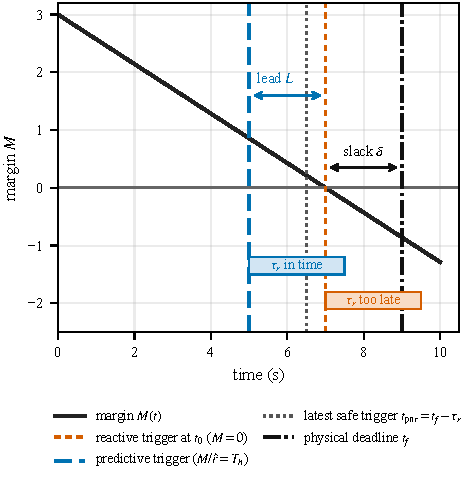
\includegraphics[width=0.72\linewidth]{fig_mechanism.pdf}
\caption{The unpadded reactive rule fires at margin expiry, while the predictive rule fires $L$ seconds earlier. The earlier trigger changes the recovery outcome only when $\delta<\tau_r\le\delta+L$.}
\label{fig:mech}
\end{figure}

\section{Evaluation Methodology}\label{sec:method}

\paragraph{Single-margin simulator and stopping deadlines.}
The single-margin experiment models two robots on perpendicular paths. Robot A may brake and wait for robot B; an optimistic, range-dependent bias hides the conflict and additive Gaussian measurement noise perturbs the monitored margin. The bias is proportional to $\mathrm{range}^{p}$: $p<1$ reveals the conflict late, $p=1$ gives a linear reveal, and $p>1$ reveals it earlier. Recovery is rate-limited braking with capability $a_{\max}$. The predictive rule estimates the margin slope with a Theil--Sen estimator over the latest eight samples. To avoid division by a fitted slope near zero, the implementation requires a decay magnitude greater than $10^{-3}$ margin units per second; otherwise the predictive rule uses its $M\le0$ fallback.

A general point-of-no-return procedure could replay the realized future from every recorded state and determine the last state from which an admissible recovery avoids failure. We use two model-specific quantities and do not treat either as a general safety certificate. First, a continuous-time braking calculation gives the latest trigger that would stop A outside the wider crossing zone. It is conservative relative to the simulator's collision condition: with the default parameters it is $8.65$\,s ($8.6$\,s to one decimal). Second, deterministic replay on the simulator's $0.1$\,s control grid finds $8.8$\,s as the latest tested forced-trigger instant that avoids a collision in the default conflict episode. The latter is an empirical, grid-dependent boundary, not a continuous-time proof.

\paragraph{Exploratory single-margin sweeps.}
The dose-response experiment compares an uncertainty-blind arrival-gap trigger, the current-margin trigger at $M=0$, and prediction. It uses 40 paired noise seeds at each of seven severities, with the predictive horizon fixed at $T_h=2.0$\,s. The recovery-capability and degradation-shape sweeps use 25 paired seeds at each of five severities, or 125 episodes per plotted setting and method. For each setting, the fixed-pad candidates are
\[
  \rho\in\{0,0.5,1.0,1.5,2.0,2.5,3.0,4.0\}.
\]
The displayed comparator is the candidate with the lowest mean successful elapsed time among those for which every episode succeeds on that same setting and seed grid. Selection and reporting therefore use the same simulations. These figures are exploratory mechanism checks, not out-of-sample performance estimates.

\section{Experiments}\label{sec:exp}

\paragraph{Untuned baselines favor early triggering (Figure~\ref{fig:dose}).}
Against an uncertainty-blind current-gap rule and an unpadded current-margin rule, the $T_h=2.0$\,s predictive rule appears strong. With rate-limited recovery ($a_{\max}=1.0$), the uncertainty-blind rule fails first as fault severity grows, the unpadded rule collides in many moderate- and high-severity episodes, and the predictive rule records no collisions on this exploratory seed grid. This shows that earlier action can matter in the simulator, but not that prediction is needed; a padded current-margin rule can also act early.

\begin{figure}[tbp]
\centering
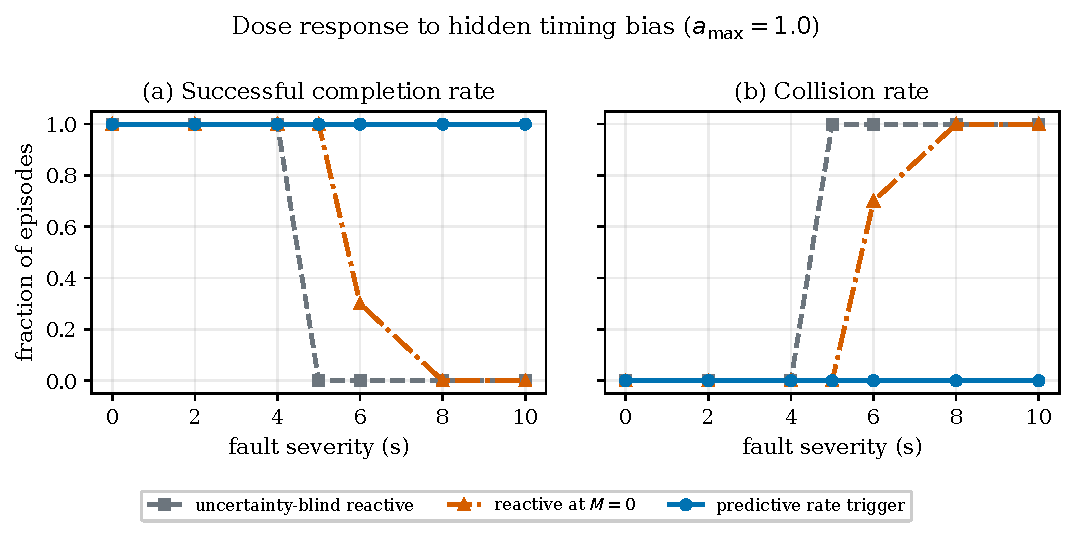
\includegraphics[width=\linewidth]{fig_dose.pdf}
\caption{Exploratory single-margin dose response with $T_h=2.0$\,s and rate-limited recovery. Results are observed rates over 40 paired noise seeds per severity. Figure~\ref{fig:boundary} adds an in-sample fixed-pad comparison.}
\label{fig:dose}
\end{figure}

\paragraph{Exploratory sweeps locate a narrow observed boundary (Figure~\ref{fig:boundary}).}
The plotted difference is the selected fixed-pad mean elapsed time minus the predictive mean, so positive values favor prediction. The fixed pad is selected in-sample at every setting. Under the slowest recovery ($a_{\max}=0.5$), the predictive rule finishes about $0.56$\,s sooner; the sign changes as recovery becomes faster, reaching $-1.31$\,s at $a_{\max}=3.0$. In the degradation-shape sweep at slow recovery, the predictor records collisions at $p=0.3$ and $p=0.5$, is about $1.23$\,s faster at $p=0.7$, and is slower than the selected fixed pad from $p=0.9$ onward. These differences are small relative to missions of roughly 25--30\,s, and the selection procedure does not support inferential claims.

\begin{figure}[tbp]
\centering
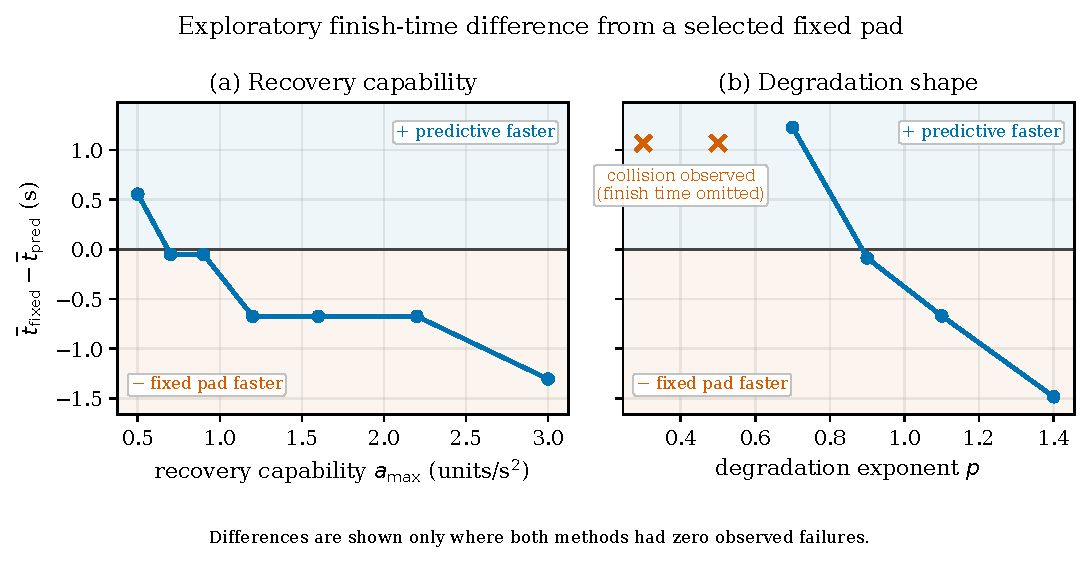
\includegraphics[width=\linewidth]{fig_boundary.pdf}
\caption{Exploratory elapsed-time difference between the $T_h=2.0$\,s predictive rule and the fixed pad selected on the same runs. Positive values favor prediction. Crosses replace timing comparisons where the predictive rule records a collision.}
\label{fig:boundary}
\end{figure}

\paragraph{Held-out tuning changes the comparison (Table~\ref{tab:heldout-single}).}
The finer, equal-budget searches select $\rho=2.5$ and $T_h=2.5$\,s. On the 6,750 held-out conflict episodes, the fixed rule succeeds in all 6,750 and records no collision. The tuned predictive rule succeeds in 6,748 and records two collisions, one at each of the two highest severities for $a_{\max}=0.5$ and $p=0.7$. Its successful-only mean elapsed time is $26.577$\,s, compared with $27.690$\,s for the fixed rule. These means condition on different success sets. Accordingly, we do not attach a paired interval or claim an efficiency advantage. For context, retaining the exploratory $T_h=2.0$\,s horizon on the same held-out conflict set gives 172 collisions in 6,750 episodes and 6,578 successful episodes; its successful-only mean is $25.990$\,s.

In the 2,250 held-out clear episodes, both tuned arms complete without collision. The fixed rule yields unnecessarily in $1800/2250$ episodes (80.0\%), while the predictive rule does so in $1358/2250$ (60.36\%). This is evidence of fewer interventions in the specified clear grid, not a safety-adjusted performance win. The maximum exact-scenario upper endpoint among the pointwise 95\% Wilson collision intervals is $0.0250$ for the fixed rule and $0.0368$ for the predictive rule. Taking the maximum does not turn those intervals into a simultaneous guarantee.

\begin{table}[tbp]
\centering
\small
\caption{Seed-disjoint single-margin test results. Elapsed time is averaged over successful conflict episodes only.}
\label{tab:heldout-single}
\begin{tabular}{lcccc}
\toprule
Arm & Parameter & Collisions & Successes & Mean time (s) \\
\midrule
Fixed margin & $\rho=2.5$ & $0/6750$ & $6750/6750$ & $27.690$ \\
Predictive, tuned & $T_h=2.5$ & $2/6750$ & $6748/6750$ & $26.577$ \\
Predictive, retained & $T_h=2.0$ & $172/6750$ & $6578/6750$ & $25.990$ \\
\bottomrule
\end{tabular}
\end{table}

\section{Discussion}\label{sec:disc}

Before implementing prediction, one can first ask whether its lead changes what recovery can accomplish. Prediction is most plausible when recovery is slow enough for an earlier trigger to cross the boundary in Proposition~\ref{prop:boundary}, and when degradation rates vary in a way that can be estimated before that boundary. At one known constant rate, a fixed pad reproduces the studied predictive trigger. Under fast, committed serialization, tuning may remove predictive lead altogether.

The simulators produce different results. In the single-margin study, the exploratory figures favor prediction over the unpadded rules and, in a few settings, over the in-sample fixed pad. After equal-budget, seed-disjoint tuning, the predictive arm intervenes less often on clear paths and has a lower descriptive successful-only elapsed time. It also records two held-out conflict collisions where the fixed arm records none, so an efficiency comparison at matched outcomes is unavailable. In the coordination study, both tuned arms succeed throughout the held-out conflict grid and the predictive arm finishes earlier. Its lower rate of clear-path serialization is consistent with adaptation to degradation rate.

The coordination result depends on the recovery design. The first trigger commits one total order, after which blockers and release events determine the motion. Prediction changes when this commitment occurs; the order is never revised. The paired interval thus describes variation over measurement noise on the fixed 27-scenario grid. It says nothing about unseen geometries, robot counts, dynamics, or online re-planning.

Proposition~\ref{prop:reduction} also suggests an intermediate design: scale a current-margin threshold using an online rate estimate, without constructing a larger predict-then-recover stack. Its practical value would still depend on estimator delay, noise, and changes in degradation rate.

Zero observed collisions is not a safety guarantee. The pointwise Wilson intervals are not simultaneous bounds over the scenario family, and holding out noise seeds does not create a new population of robot environments. The v1 comparison accordingly tunes the simpler early-trigger baseline, verifies that untreated paths conflict, separates tuning from testing, and reports failures before conditional timing.

\section{Limitations and Version Scope}\label{sec:limits}

The v1 evidence comes from controlled two-dimensional point-kinematic simulators, scalar monitored margins, fixed scenario grids, Gaussian measurement noise, and one braking or serialization recovery family. It does not cover vehicle dynamics, perception failures, localization, networking, asynchronous execution, or a full navigation stack. The analytical stopping deadline is deliberately conservative, while the replay-derived $8.8$\,s deadline is empirical for one deterministic episode and a $0.1$\,s trigger grid.

The dose-response and boundary figures are exploratory: fixed-pad selection and reporting use the same runs, and the predictive horizon remains at $2.0$\,s. The second single-margin experiment separates tuning and test seeds and gives both methods the same candidate grid, but only noise realizations are held out. The simulator, factor levels, and selection rule are fixed rather than sampled from a target population. Its reported Wilson intervals are pointwise, and their largest upper endpoint is not a simultaneous confidence bound. Because the held-out primary arms have different collision outcomes, their conditional completion times are descriptive and no inferential efficiency comparison is made.

In the coordination simulator, untreated conflict trajectories physically overlap, and waiting robots have explicit blockers and release conditions. The first trigger nevertheless commits an immutable ordering; the simulator does not re-plan. The observed timing advantage therefore concerns this one-shot serialization rather than multi-robot coordination in general. The bootstrap interval varies measurement noise over a fixed 27-scenario grid and does not cover new geometries, dynamics, robot counts, or degradation families. The no-intervention arm consumes no measurement noise, so repeated runs within a physical scenario are deterministic duplicates rather than independent safety evidence. The model contains only three robots and one shared zone.

ROS~2/Nav2 experiments with localization degradation, communication faults, planner interactions, and full-stack telemetry are reserved for v2; no v1 claim extends to them. The related-work search is targeted rather than systematic. A later archival submission should broaden and document the search and recheck each citation against its surrounding claim.

\section{What I take from this}
\label{sec:conclusion}

For the trigger studied here, prediction is a way to adapt a margin threshold
to the estimated rate of decline.  Its value depends on whether the extra lead
changes what recovery can accomplish and how much unnecessary early action it
avoids.  In the timing model, recovery duration and deadline slack set that
boundary, and observation age consumes the available lead one for one.

The three-robot experiment shows a practical benefit of this adaptation.  Both
tuned rules succeed in all 1,620 conflict episodes, while prediction reduces
mean completion time by $2.779$\,s (paired 95\% interval
$[2.659,2.902]$\,s).  It also cuts unnecessary clear-path serializations from
1,080 to 21 out of 1,620 episodes.  Waiting until closer to the point when
recovery is needed saves time in this fixed-order crossing setup.

The two-robot experiment shows why the rate estimate matters.  The tuned fixed
rule records $0/6750$ conflict collisions and prediction records $2/6750$, both
where the conflict is revealed late and braking is slow.  A rate estimate that
lags a steepening decline can use up the lead the predictive rule was meant to
provide.

My takeaway is that the recovery requirement is the right place to start.
When recovery needs similar lead times across cases but margins decline at
different rates, adapting the threshold can reduce unnecessary waiting.
Observation delay and changing recovery durations are the next variables I
would test, using the tuned fixed threshold as the baseline.

\emph{Code and data.}  The simulators, tests, episode-level results, and figure
scripts are available at \url{\repositoryurl}.


\bibliographystyle{IEEEtran}
\bibliography{references/references}

\end{document}
